\section{Algoritmi di Moorer}

In seguito alla fase di test, il passo successivo è stato quello di implementare gli algoritmi di Moorer, in quanto risultano più efficenti dei precedenti.
In questa sezione verranno inoltre inseriti i parametri ambientali ed utilizzati come controllo delle caratteristiche del riverbero. Le formule utilizzate per il calclo dei parametri sono le medesime viste nel capitolo \ref{chp:Filtri} ma con le dovute approssimazioni.

\bigskip

Il codice seguente descrive il filtro All Pass secondo le indicazioni di Moorer (visto in figura \ref{fig:apfmoorer}) e come già detto, senellisce i calcoli riducendo il numero delle moltiplicazioni ad 1.

\begin{code}
apfm(t, g) = _<: ((+ : _*(g)),_<:_,!,_+_ : _, zm(t) : ro.cross(2))~(0 -_) : +
with{
    zm(t) = de.delay(ma.SR,t);
};
\end{code}

\bigskip

Il grafico risultante è in figura \ref{fig:apfmoorerfaust}

\begin{figure}[htp]
\centering
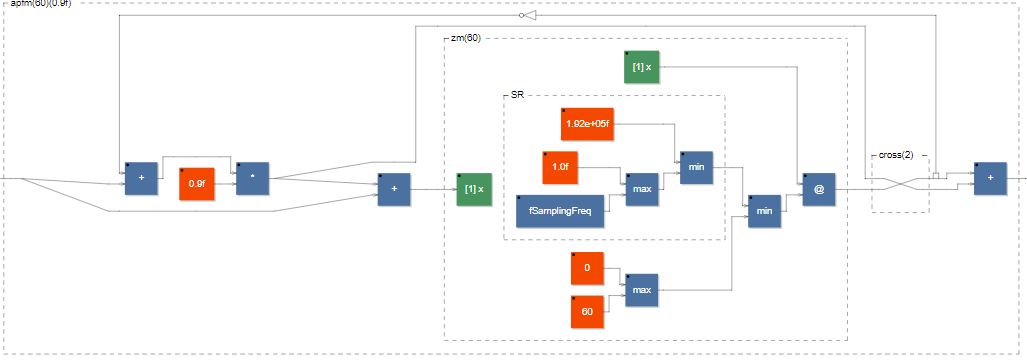
\includegraphics[width=%
1.2\textwidth]{apfmoorerfaust}
\caption{All Pass descritto da Moorer}
\label{fig:apfmoorerfaust}
\end{figure}
